\section{Experiments}
\label{sec:experiments}

We evaluate the three families of geometric attribution algorithms proposed in this paper. They share the same cooperative game, value functions and link functions, and differ only in where the vectors of the Gram matrix come from:
\begin{itemize}
    \item \textbf{EATT} embeds the snippets and the response with an external text encoder (Section~\ref{subsec:geometric_values});
    \item \textbf{GATT} builds one vector per player from the queries, keys and logits of the LLM, i.e., from \emph{where} the response attends (Section~\ref{sec:attention_gram_attribution});
    \item \textbf{VATT} represents every snippet by the subspace spanned by its value vectors and the response by what it reads from the context, i.e., by \emph{what} the attention moves (Section~\ref{sec:set_embeddings}).
\end{itemize}
All three need at most two LLM forward passes per instance. We compare them with perturbation-based and gradient-based baselines on multi-hop question answering (HotpotQA, 2WikiMultihopQA, MuSiQue), summarization (CNN/DailyMail) and two redundancy variants of HotpotQA, and ask four questions. (i) How closely do they agree with exact likelihood Shapley values~\cite{nematov2025source}? (ii) Do they assign credit to the snippets that actually support the answer? (iii) How do they trade off accuracy against the number of LLM passes, and how does this change with the number of snippets, the task and redundancy among the snippets? (iv) How do the value function, the link function and the hyperparameters affect (i) and (ii)?

\subsection{Experimental Setup}
\label{subsec:exp_setup}

\paragraph{Benchmarks.}
We evaluate on six benchmark settings that differ in the number of snippets, the availability of an exact reference, the presence of supporting-fact labels and the redundancy among snippets (Table~\ref{tab:exp_benchmarks}). All instances are sampled uniformly at random with a fixed seed; every paragraph or sentence is one snippet, prefixed with its title where available.
\begin{itemize}
    \item \textbf{HotpotQA}~\cite{yang2018hotpotqa} (distractor setting, development split), following ContextCite~\cite{cohen2024contextcite}. Every question comes with ten Wikipedia paragraphs, two of which are annotated as \emph{supporting facts}; both are needed for the two-hop reasoning chain. We keep both supporting paragraphs and the first four distractors in their original order ($n = 6$; one instance has only two paragraphs) and truncate each paragraph at $1000$ characters. The distractors are retrieved for lexical overlap with the question and often mention its entities. HotpotQA is the main benchmark ($200$ instances); all ablations in Sections~\ref{subsec:exp_values}--\ref{subsec:exp_cost} use it.
    \item \textbf{2WikiMultihopQA}~\cite{ho2020constructing} (development split, $100$ instances) has the same format with ten paragraphs, of which two to four are supporting facts (compositional, comparison, inference and bridge-comparison questions). We keep all ten paragraphs ($n = 10$), so exact enumeration needs $2^{10} = 1024$ coalitions per instance.
    \item \textbf{MuSiQue}~\cite{trivedi2022musique} (answerable split, development set, $80$ instances) composes two to four single-hop questions into one, so that two to four of its $20$ paragraphs are supporting facts and the others are retrieved distractors. We keep all twenty paragraphs ($n = 20$); exact enumeration ($2^{20}$ coalitions) is infeasible, and this benchmark tests how the methods scale with $n$. Answers are matched against the gold answer and its aliases.
    \item \textbf{CNN/DailyMail}~\cite{nallapati2016abstractive} (version 3.0.0, test split, $100$ articles), the summarization benchmark of ContextCite. The snippets are the first $n = 20$ sentences of each article (articles with fewer than $10$ sentences are skipped), and the instruction asks for a summary of at most three sentences. There are no supporting-fact labels; we evaluate only agreement and ablation faithfulness.
    \item \textbf{Duplicated HotpotQA} and \textbf{paraphrased HotpotQA} ($100$ instances each) test redundancy. We take $100$ of the HotpotQA instances and insert a copy of the first supporting paragraph at a random position that is not adjacent to the original ($n = 7$). In the duplicated variant the copy is verbatim; in the paraphrased variant the model itself rewrites it (\emph{``Paraphrase the following paragraph. Keep every fact, name, date and number, but change the wording and the sentence structure''}, greedy decoding). A faithful attribution method should split the credit between the two copies; leave-one-out cannot, because removing either copy leaves the other in the context.
\end{itemize}

\begin{table}[t]
\centering
\small
\setlength{\tabcolsep}{3pt}
\begin{tabular}{lllrrlrrc}
\toprule
Benchmark & Task & $n$ & Inst. & Supp. & Reference & Coal. & Correct (\%) & $\bar w$ \\
\midrule
HotpotQA & 2-hop QA & 6 & 200 & 2 & exact & 64 & 80.0 & 0.95 \\
2WikiMultihopQA & 2--4-hop QA & 10 & 100 & 2--4 & exact & 1024 & 78.0 & 0.98 \\
MuSiQue & 2--4-hop QA & 20 & 80 & 2--4 & ContextCite-128 & 302 & 55.0 & 0.97 \\
CNN/DailyMail & summarization & $\le 20$ & 100 & -- & ContextCite-128 & 298 & -- & 0.99 \\
HotpotQA + duplicate & 2-hop QA & 7 & 100 & 3 & exact & 127 & 82.0 & 0.96 \\
HotpotQA + paraphrase & 2-hop QA & 7 & 100 & 3 & exact & 127 & 80.0 & 0.96 \\
\bottomrule
\end{tabular}
\caption{Benchmarks. \emph{Supp.:} supporting facts per instance; \emph{Coal.:} mean number of coalitions whose $v_{\text{LL}}$ is evaluated per instance (all $2^n$ for the exact reference; for $n = 20$, the union of the coalitions queried by the baselines, the $128$ reference masks and the $64$ LDS masks); \emph{Correct:} responses that contain the gold answer or an alias; $\bar w$: mean global context weight.}
\label{tab:exp_benchmarks}
\end{table}

\paragraph{Model and responses.}
We use the instruction-tuned Gemma~4 31B dense model~\cite{gemma4}. It has $L = 60$ layers, of which $|\mathcal{L}_{\text{glob}}| = 10$ are global attention layers ($\ell \in \{5, 11, \dots, 59\}$); the remaining layers use a sliding window and cannot route information from distant snippets to the response (Section~\ref{subsec:attention_notation}). Each global layer has $32$ query heads that share $4$ KV heads, with key and value dimension $512$. The prompt $p$ consists of a fixed task instruction (\emph{``Answer the question concisely using only the provided context snippets''} for QA, the summarization instruction above for CNN/DailyMail), the numbered snippets and the question, formatted with the chat template of the model. The response $r$ is generated by the model itself with greedy decoding (at most $64$ tokens for QA and $96$ for summarization), so all methods explain the response the model actually produced. Table~\ref{tab:exp_benchmarks} lists the fraction of responses that contain the normalized gold answer; in most of the other QA instances the model states that the context is insufficient. Because supporting-fact labels strictly apply only to correct answers, we also report all results on the answer-correct instances (Appendix~\ref{app:exp_correct}).

\paragraph{Reference attribution.}
When $n \le 10$ (HotpotQA, 2WikiMultihopQA and both redundancy variants), we evaluate the likelihood game of~\cite{nematov2025source}, $v_{\text{LL}}(S') = \log P(r \mid p, S') - \log P(r \mid p, \emptyset)$, \emph{exactly} on all $2^n$ coalitions and map the exact Shapley vector to the simplex with the rectified link; this reference is free of Monte Carlo noise. On HotpotQA this takes $63.7$ teacher-forced forward passes and $8.3$\,s per instance on $8$ TPU v6e chips. For $n = 20$ (MuSiQue and CNN/DailyMail), we use ContextCite~\cite{cohen2024contextcite} with a high budget of $B = 128$ random ablation masks as the reference, i.e., four times the budget of the ContextCite baseline below, and on MuSiQue we additionally rely on the supporting-fact labels, which do not depend on any reference. Since all methods share the same global context weight $w$ in the final attribution $\boldsymbol{\alpha} = w \cdot g(\boldsymbol{\phi})$ (Definition~\ref{def:attribution_algorithm}), we compare the snippet distributions $g(\boldsymbol{\phi}) \in \Delta^{n-1}$. The responses rely almost entirely on the context ($w \ge 0.95$ on average on every benchmark, Table~\ref{tab:exp_benchmarks}).

\paragraph{Proposed geometric methods.}
Each method below is evaluated with the value functions of Sections~\ref{subsec:geometric_values} and~\ref{subsec:set_values}. Apart from the empty-context pass on $(p, \emptyset, r)$ that is shared by all methods for $w$, GATT and VATT need one teacher-forced pass on $(p, S, r)$, which can be the generation pass itself.
\begin{itemize}
    \item \textbf{EATT (Gecko).} Snippets and response are embedded with the Gecko encoder~\cite{lee2024gecko} ($1$B parameters, $d = 768$) and normalized; the $(n+1) \times (n+1)$ Gram matrix $\mathbf{G}^{+}_{\{[n]\}}$ is formed as in Section~\ref{subsec:geometric_values}.
    \item \textbf{GATT-RCB} and \textbf{GATT-TCR.} The Gram matrices of Section~\ref{subsec:two_grams}, computed from the queries, keys and pre-softmax logits of the $m = 10 \cdot 32$ global heads. Unless stated otherwise, $k_0 = 2$ and $\kappa = 0.9$.
    \item \textbf{VATT.} In every global head $\nu$, snippet $s_i$ is represented by the top-$k$ eigenvectors of its attention-weighted value covariance $\sum_{c \in \mathcal{T}_i} \bar{a}^\nu_c \mathbf{v}^\nu_c \mathbf{v}^{\nu\top}_c$ (rank truncation, Section~\ref{subsec:set_regularization}), and the response by its context read-outs $\mathbf{y}^\nu_t$ (Section~\ref{subsec:vatt}) and, for the principal-angle value functions, by their top-$k_r$ eigenvectors. Heads are combined as a direct sum: $v_{\text{proj}}$ is energy-weighted over heads~\eqref{eq:vatt_proj}, $v_{\text{logvol}}$ is summed, and $v_{\text{vol}}$ and $v_{\text{ent}}$ are averaged over heads (the direct-sum volume is a product of $320$ factors and numerically zero). Unless stated otherwise, $k = k_r = 4$.
\end{itemize}
$v_{\text{logvol}}$ uses $\lambda = 10^{-3}$. For EATT and GATT, Shapley values are estimated with $K = 100$ random permutations ($15$--$30$\,ms per instance on CPU, Section~\ref{subsec:exp_cost}). VATT tabulates its value function on the coalitions it needs, so for $n \le 10$ we compute exact Shapley values and for $n = 20$ we use $K = 50$ permutations. Unless stated otherwise, we report the floor-shifted power link $g^{\text{fl},2}$ of Section~\ref{subsec:contrast_calibration}; Section~\ref{subsec:exp_values} compares it with the rectified link.

\paragraph{Perturbation and gradient baselines.}
Four baselines perturb the snippet set and reuse memoized evaluations of $v_{\text{LL}}(S')$, so their budgets are the exact numbers of distinct LLM forward passes:
\begin{itemize}
    \item \textbf{ContextCite}~\cite{cohen2024contextcite}: sparse linear surrogate (LASSO, penalty $0.01\,\operatorname{sd}(y)$) fitted on $B = 32$ uniform random ablation masks ($25.1$ distinct coalitions on average for $n = 6$).
    \item \textbf{KernelSHAP}~\cite{lundberg2017unified}: least-squares surrogate under the Shapley kernel with the efficiency constraint ($B = 32$: $\emptyset$, $[n]$ and $30$ sampled coalitions).
    \item \textbf{Permutation Shapley (LLH-Perm)}~\cite{castro2009polynomial}: $K$ permutations of $v_{\text{LL}}$ (Lemma~\ref{lemma:unbiased_estimator}); $K = 10$ for $n \le 10$ and $K = 2$ ($2n$ passes) for $n = 20$.
    \item \textbf{Leave-One-Out (LOO)}~\cite{liu2025attribot}: $\phi_i = v_{\text{LL}}([n]) - v_{\text{LL}}([n] \setminus \{i\})$ ($n + 2$ passes including $\emptyset$).
\end{itemize}
Two baselines differentiate $F(\mathbf{x}) = \log P(r \mid \mathbf{x})$ with respect to the token embeddings (Section~\ref{subsec:gradient_view}) and sum token scores within each snippet: \textbf{Gradient $\times$ Input}~\cite{simonyan2014deep} ($1$ forward-backward pass, baseline $\mathbf{x}'$ replaces snippet tokens with the $\langle\text{pad}\rangle$ embedding) and $16$-step \textbf{Integrated Gradients}~\cite{sundararajan2017axiomatic} along $\mathbf{x}' + \alpha(\mathbf{x} - \mathbf{x}')$ ($16$ forward-backward passes). Perturbation and gradient scores are already centered at zero for irrelevant snippets, so we use the rectified link for them (floor-shifting yields similar or lower rank correlation for all six). The direct attention heuristics Citation and Easton V2.1 are evaluated separately in Section~\ref{subsec:exp_citation_easton}.

\paragraph{Metrics.}
All metrics are computed within each instance over its $n$ snippets and averaged over instances, with $95\%$ bootstrap confidence intervals ($2000$ resamples).
\begin{itemize}
    \item \emph{Agreement with the reference:} Pearson $r$, Spearman $\rho$, Kendall $\tau_b$, mean absolute error (MAE, in percentage points) and top-1 agreement.
    \item \emph{Supporting facts:} supporting-fact mass $\sum_{i \in S_{\text{supp}}} g_i(\boldsymbol{\phi})$, AUROC for the binary supporting-fact label, and precision@$k$ (P@$k$) with $k = |S_{\text{supp}}|$ (P@2 on HotpotQA).
    \item \emph{Ablation faithfulness}, which needs no labels and follows ContextCite and AT2~\cite{cohen2024contextcite,cohenwang2025learning}: the \emph{top-$k$ log-probability drop} $v_{\text{LL}}([n]) - v_{\text{LL}}([n] \setminus T_k)$, where $T_k$ holds the $k$ snippets with the largest attribution ($k \in \{1, 2, 3\}$ for $n \le 10$ and $\{1, 3, 5\}$ for $n = 20$; higher is better), and the \emph{linear datamodeling score} (LDS), the Spearman correlation between the additive prediction $\sum_{i \in S'} g_i(\boldsymbol{\phi})$ and $v_{\text{LL}}(S')$ over all $2^n$ coalitions for $n \le 10$ or over $64$ random half-size masks for $n = 20$. Every coalition is scored with an additional teacher-forced pass that is not counted towards the budget of any method.
    \item \emph{Redundancy} (duplicated and paraphrased HotpotQA): the credit on the original and its copy, the \emph{split ratio} $\min(\alpha_o, \alpha_c) / (\alpha_o + \alpha_c)$ ($0.5$ is an even split), and the fraction of instances in which one copy receives less than $1\%$ of their joint credit or both together receive less than $1\%$ of the total.
\end{itemize}

\subsection{Main Results}
\label{subsec:exp_main}

Table~\ref{tab:exp_main} compares the best configuration of every geometric family with all baselines on HotpotQA; Section~\ref{subsec:exp_multi} repeats the comparison on the other benchmarks. The full grid of value functions follows in Section~\ref{subsec:exp_values}.

\begin{table}[t]
\centering
\small
\setlength{\tabcolsep}{2.6pt}
\resizebox{\linewidth}{!}{%
\begin{tabular}{lllcccccccccc}
\toprule
 & & & & \multicolumn{5}{c}{Agreement with Exact LLH-Shapley} & \multicolumn{3}{c}{Supporting facts} \\
\cmidrule(lr){5-9} \cmidrule(lr){10-12}
Method & $v$ & Link & Passes & Pearson $r$ & Spearman $\rho$ & Kendall $\tau$ & MAE (pp) $\downarrow$ & Top-1 (\%) & Mass (\%) & AUROC & P@2 (\%) \\
\midrule
\multicolumn{12}{l}{\emph{Proposed geometric methods (two LLM passes)}} \\
EATT (Gecko) & $v_{\mathrm{logvol}}$ & floor & $2^\dagger$ & 0.75{\scriptsize$\pm$0.05} & 0.68{\scriptsize$\pm$0.03} & 0.59{\scriptsize$\pm$0.03} & 10.3{\scriptsize$\pm$1.2} & 70.0{\scriptsize$\pm$6.2} & \textbf{92.3}{\scriptsize$\pm$1.9} & 0.91{\scriptsize$\pm$0.02} & 83.2{\scriptsize$\pm$3.4} \\
GATT-RCB & $v_{\mathrm{logvol}}$ & floor & 2.0 & 0.72{\scriptsize$\pm$0.05} & 0.60{\scriptsize$\pm$0.04} & 0.51{\scriptsize$\pm$0.04} & 11.7{\scriptsize$\pm$1.3} & 67.0{\scriptsize$\pm$6.5} & 75.4{\scriptsize$\pm$3.1} & 0.83{\scriptsize$\pm$0.03} & 70.8{\scriptsize$\pm$4.0} \\
GATT-TCR & $v_{\mathrm{logvol}}$ & floor & 2.0 & 0.78{\scriptsize$\pm$0.04} & 0.62{\scriptsize$\pm$0.04} & 0.53{\scriptsize$\pm$0.03} & 10.2{\scriptsize$\pm$1.3} & 75.5{\scriptsize$\pm$5.8} & 78.1{\scriptsize$\pm$3.0} & 0.83{\scriptsize$\pm$0.03} & 68.0{\scriptsize$\pm$3.6} \\
VATT & $v_{\mathrm{proj}}$ & floor & 2.0 & \textbf{0.91}{\scriptsize$\pm$0.03} & 0.78{\scriptsize$\pm$0.02} & 0.69{\scriptsize$\pm$0.02} & \textbf{5.8}{\scriptsize$\pm$0.8} & \textbf{82.0}{\scriptsize$\pm$5.2} & 91.5{\scriptsize$\pm$2.0} & \textbf{0.93}{\scriptsize$\pm$0.02} & \textbf{87.8}{\scriptsize$\pm$3.1} \\
VATT & $v_{\mathrm{vol}}$ & rect. & 2.0 & 0.89{\scriptsize$\pm$0.03} & \textbf{0.84}{\scriptsize$\pm$0.03} & \textbf{0.79}{\scriptsize$\pm$0.03} & 6.9{\scriptsize$\pm$0.9} & 78.5{\scriptsize$\pm$5.8} & 91.1{\scriptsize$\pm$2.4} & 0.91{\scriptsize$\pm$0.02} & 84.5{\scriptsize$\pm$3.5} \\
\midrule
\multicolumn{12}{l}{\emph{Gradient and subset-ablation baselines}} \\
Gradient $\times$ Input & $\nabla F$ & rect. & $2.0^\ddagger$ & $-0.01${\scriptsize$\pm$0.06} & $-0.01${\scriptsize$\pm$0.06} & $-0.01${\scriptsize$\pm$0.05} & 26.0{\scriptsize$\pm$1.3} & 18.5{\scriptsize$\pm$5.2} & 30.4{\scriptsize$\pm$4.3} & 0.49{\scriptsize$\pm$0.03} & 30.0{\scriptsize$\pm$4.1} \\
Integrated Gradients (16) & $\nabla F$ & rect. & $17.0^\ddagger$ & 0.07{\scriptsize$\pm$0.06} & 0.10{\scriptsize$\pm$0.06} & 0.09{\scriptsize$\pm$0.06} & 24.1{\scriptsize$\pm$1.1} & 17.0{\scriptsize$\pm$5.0} & 36.8{\scriptsize$\pm$4.5} & 0.54{\scriptsize$\pm$0.03} & 35.2{\scriptsize$\pm$4.1} \\
LOO & $v_{\mathrm{LL}}$ & rect. & 8.0 & 0.97{\scriptsize$\pm$0.01} & 0.77{\scriptsize$\pm$0.03} & 0.71{\scriptsize$\pm$0.03} & 3.3{\scriptsize$\pm$0.5} & 95.5{\scriptsize$\pm$2.8} & 92.9{\scriptsize$\pm$2.4} & 0.90{\scriptsize$\pm$0.02} & 84.5{\scriptsize$\pm$3.4} \\
KernelSHAP (32) & $v_{\mathrm{LL}}$ & rect. & 23.3 & 0.91{\scriptsize$\pm$0.02} & 0.79{\scriptsize$\pm$0.03} & 0.73{\scriptsize$\pm$0.03} & 5.8{\scriptsize$\pm$0.7} & 83.5{\scriptsize$\pm$5.0} & 84.6{\scriptsize$\pm$2.5} & 0.85{\scriptsize$\pm$0.03} & 75.0{\scriptsize$\pm$3.6} \\
ContextCite (32) & $v_{\mathrm{LL}}$ & rect. & 25.1 & 0.99{\scriptsize$\pm$0.01} & 0.90{\scriptsize$\pm$0.02} & 0.86{\scriptsize$\pm$0.02} & 2.5{\scriptsize$\pm$0.3} & 94.5{\scriptsize$\pm$3.2} & 92.0{\scriptsize$\pm$2.1} & 0.90{\scriptsize$\pm$0.02} & 84.0{\scriptsize$\pm$3.5} \\
LLH-Perm ($K=10$) & $v_{\mathrm{LL}}$ & rect. & 34.9 & 0.97{\scriptsize$\pm$0.01} & 0.89{\scriptsize$\pm$0.02} & 0.86{\scriptsize$\pm$0.03} & 2.7{\scriptsize$\pm$0.4} & 88.5{\scriptsize$\pm$4.5} & 93.0{\scriptsize$\pm$2.4} & 0.88{\scriptsize$\pm$0.02} & 80.8{\scriptsize$\pm$3.6} \\
\midrule
Exact LLH-Shapley (ref.) & $v_{\mathrm{LL}}$ & rect. & 63.7 & 1 & 1 & 1 & 0 & 100 & 94.6 & 0.91 & 84.8 \\
Uniform & -- & -- & 0 & -- & -- & -- & 23.7 & 11.5 & 33.7 & 0.50 & 20.5 \\
\bottomrule
\end{tabular}%
}
\caption{Attribution quality on $200$ HotpotQA instances (Gemma~4 31B, $n = 6$ snippets, $2$ supporting facts per instance). Mean over instances $\pm$ half-width of the $95\%$ bootstrap confidence interval. \emph{Passes:} mean distinct LLM passes per instance ($^\dagger$only needed for $w$, plus $n+1$ Gecko encoder calls; $^\ddagger$includes $1$ or $16$ forward-backward passes). VATT uses $k = k_r = 4$. Best entry among the proposed methods is in bold.}
\label{tab:exp_main}
\end{table}

\paragraph{Where the geometry comes from matters most.}
All three families agree with exact likelihood Shapley values far better than uniform attribution (MAE $23.7$\,pp) without ablating a single snippet, but the source of the vectors makes a large difference. EATT and GATT reach Pearson $r = 0.72$--$0.78$ and MAE $10.2$--$11.7$\,pp. VATT reaches $r = 0.91$ and MAE $5.8$\,pp, halving the error of the other two families. With $v_{\text{vol}}$ and the rectified link, it also reaches the highest rank agreement of any two-pass method ($\rho = 0.84$, $\tau = 0.79$). The value vectors are the representations through which the snippets actually influence the response, so a geometry built on them inherits the routing of the model; Gecko cosines describe semantic similarity, and the query--key constructions of GATT describe where the response looks, not what it receives.

\paragraph{Supporting facts.}
EATT and VATT recover the supporting facts as well as the exact reference or better: EATT places $92.3\%$ of the credit on them (AUROC $0.91$, P@2 $83.2\%$), and VATT $91.5\%$ (AUROC $0.93$, P@2 $87.8\%$), compared with $94.6\%$, $0.91$ and $84.8\%$ for exact LLH-Shapley. GATT is weaker at its pre-specified hyperparameters ($75.4$--$78.1\%$ mass, AUROC $0.83$) but closes most of the gap with larger anchor sets (AUROC $0.88$ at $k_0 = 8$, Section~\ref{subsec:exp_sensitivity}). The ordering EATT $>$ GATT follows the similarity structure of the Gram matrices: Gecko cosines between snippets (median $0.47$) separate complementary supporting facts from entity-overlapping distractors more sharply than the nearly orthogonal RCB vectors (median $0.11$) or the background-dominated TCR profiles (median $0.84$).

\paragraph{Accuracy versus cost.}
Figure~\ref{fig:exp_budget} places the methods on the accuracy--cost plane. Methods that query $v_{\text{LL}}(S')$ converge to the reference as their budget grows; ContextCite is the most sample-efficient ($r = 0.86$ at $7.6$ passes, $0.99$ at $25.1$), ahead of LLH-Perm ($0.82$ at $7.0$, $0.97$ at $34.9$) and KernelSHAP ($0.61$ at $7.6$, $0.93$ at $23.0$). LOO reaches $r = 0.97$ at $8$ passes here because the two supporting paragraphs form a \emph{complementary} chain (removing either hop breaks the answer); it assigns zero credit when evidence is duplicated across sources (Section~\ref{sec:related_work}). With two passes, VATT matches the Pearson agreement of KernelSHAP with $23.3$ passes ($r = 0.91$) and exceeds every ablation baseline, including the exact reference, in supporting-fact AUROC ($0.93$ vs.\ $0.85$--$0.91$). EATT and GATT-TCR outperform low-budget KernelSHAP ($B = 8$ and $12$) with $4\times$--$5\times$ fewer passes. Every ablation baseline scales at least linearly with $n$, whereas the geometric methods need two passes for any $n$. The gap to the ablation methods with $25$--$35$ passes ($r \ge 0.97$) remains.

\begin{figure}[t]
\centering
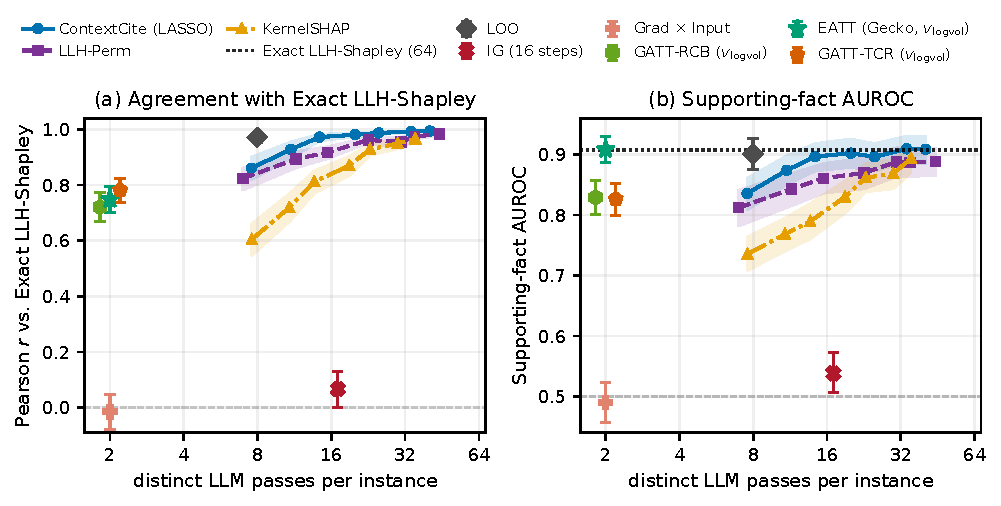
\includegraphics[width=0.95\linewidth]{figures/fig_budget_tradeoff.pdf}
\caption{Attribution accuracy versus mean distinct LLM passes per instance ($200$ HotpotQA instances; bands and error bars are $95\%$ bootstrap confidence intervals). Left: within-instance Pearson $r$ with exact $2^n$ LLH-Shapley. Right: supporting-fact AUROC. VATT ($2$ passes, $r = 0.91$, AUROC $0.93$; Table~\ref{tab:exp_main}) is not drawn.}
\label{fig:exp_budget}
\end{figure}

\paragraph{Gradient baselines fail.}
Both gradient baselines are near chance although they differentiate the exact log-likelihood: Gradient $\times$ Input reaches $r = -0.01$ and AUROC $0.49$, and Integrated Gradients $r = 0.07$ and AUROC $0.54$ at $8.0$\,s per instance. Both failures instantiate the obstructions of Section~\ref{subsec:gradient_view}. At full context, greedy responses have high token probabilities, so the prediction error $\boldsymbol{\delta}_t$ nearly vanishes (Figure~\ref{fig:snippet_gate}(d)): removing the context drops the log-likelihood by a median of $65.9$\,nats, but the $\ell_1$ norm of Gradient $\times$ Input has median $4.1$. Integrated Gradients interpolates token embeddings along a continuous ray through out-of-distribution representations, where attention routing switches abruptly, whereas the Shapley value averages discrete marginal gains along the diagonal of Owen's multilinear extension~\cite{owen1972multilinear} (Proposition~\ref{prop:owen}); its $16$-step quadrature misses the completeness identity by a median relative gap of $2.41$ ($90$th percentile $17.8$).

\subsection{Beyond HotpotQA: More Snippets, Summarization and Redundancy}
\label{subsec:exp_multi}

The HotpotQA instances have $n = 6$ complementary snippets, so exact enumeration and $25$-pass surrogates are affordable and leave-one-out is close to exact. Tables~\ref{tab:exp_multi}--\ref{tab:exp_redundancy} repeat the comparison on settings that stress each of these properties.

\paragraph{More snippets with an exact reference (2WikiMultihopQA).}
With $n = 10$ the exact reference needs $1024$ coalitions per instance, and the conclusions of HotpotQA carry over (Table~\ref{tab:exp_multi}). VATT with $v_{\text{proj}}$ reaches $r = 0.88$ and MAE $4.6$\,pp with two passes, and recovers the supporting facts as well as the exact reference (AUROC $0.99$, P@$k$ $96.0\%$ vs.\ $0.99$ and $94.5\%$); $v_{\text{vol}}$ again gives the best rank agreement of the two-pass methods ($\rho = 0.81$). GATT-TCR improves relative to HotpotQA ($r = 0.78$, AUROC $0.95$), and EATT keeps a high supporting-fact AUROC ($0.95$) despite a lower $r = 0.61$. Among the ablation baselines, KernelSHAP is the first to suffer from the larger game: with the same budget of $32$ samples, its agreement drops from $r = 0.91$ to $0.77$, and its supporting-fact AUROC ($0.89$) falls below that of every VATT variant ($0.98$--$0.99$). ContextCite ($r = 0.97$), LOO ($0.95$, $12$ passes) and LLH-Perm ($0.96$, up to $92$ passes) stay close to the reference, and both gradient baselines stay near chance ($r \le 0.20$).

\paragraph{Twenty snippets (MuSiQue).}
With $n = 20$ snippets, exact enumeration is out of reach, and the reference is ContextCite with $128$ ablations (Table~\ref{tab:exp_multi}, bottom). Because this reference is itself a sparse linear surrogate, its agreement with ContextCite with $32$ ablations ($r = 0.98$) is partly circular; the supporting-fact labels are the reference-free comparison. Here VATT with $v_{\text{logvol}}$ is the best two-pass method ($r = 0.94$, MAE $2.1$\,pp) and recovers the two to four supporting paragraphs among twenty better than the reference itself (AUROC $0.93$ vs.\ $0.90$, P@$k$ $78.5\%$ vs.\ $77.2\%$), and better than every ablation baseline, including LOO with $22$ passes (AUROC $0.89$, P@$k$ $75.8\%$) and ContextCite ($0.87$, $72.9\%$). EATT keeps a high AUROC ($0.91$) and the largest supporting-fact mass of the two-pass methods ($84.4\%$), GATT-TCR reaches $r = 0.87$, and both gradient baselines stay at chance. The fixed-budget surrogates degrade with $n$: KernelSHAP with $32$ samples falls to $r = 0.61$, AUROC $0.73$ and $37.8\%$ supporting-fact mass, and LLH-Perm with $K = 2$ ($40$ passes) to AUROC $0.86$. Rank correlations are low for every method ($\rho \le 0.53$) because most of the twenty snippets receive near-zero credit, so their order is noise. As on CNN/DailyMail, $v_{\text{vol}}$ fails on VATT with many snippets ($r = 0.31$), whereas $v_{\text{logvol}}$ improves over $v_{\text{proj}}$ ($r = 0.94$ vs.\ $0.92$, AUROC $0.93$ vs.\ $0.90$). Scoring the $302$ coalitions per instance needed for the reference, the baselines and the LDS took $120$\,s per instance; the GATT forward pass took $2.6$\,s.

\paragraph{Summarization (CNN/DailyMail).}
Summaries draw on many sentences at once, and the reference is spread accordingly (uniform attribution has MAE $6.8$\,pp). VATT with $v_{\text{logvol}}$ agrees best among the two-pass methods ($r = 0.89$, $\rho = 0.75$, MAE $2.5$\,pp, LDS $0.87$), on par with LLH-Perm with $K = 2$ ($r = 0.88$, LDS $0.87$, up to $40$ passes) and well ahead of KernelSHAP ($r = 0.67$, LDS $0.74$); ContextCite ($r = 0.94$, LDS $0.91$) and LOO ($r = 0.91$, LDS $0.89$, $22$ passes) remain the most faithful. In contrast to QA, $v_{\text{vol}}$ collapses on VATT ($r = 0.43$): summary sentences read from many overlapping value subspaces, and the volume difference, which penalizes every shared direction, assigns non-positive credit to most of them. The log-volume, whose marginal gains stay non-negative~\eqref{eq:marginal_logvol}, is the robust choice when many snippets contribute. Removing the five sentences ranked highest by VATT lowers the log-likelihood by $301$\,nats ($v_{\text{logvol}}$; $314$ for the reference and $304$ for ContextCite), against $251$ for the first five sentences of the article (Table~\ref{tab:exp_faithfulness}).

\paragraph{Ablation faithfulness.}
Table~\ref{tab:exp_faithfulness} reports the label-free metrics of ContextCite and AT2. They reproduce the ordering of the agreement metrics on every benchmark. VATT reaches LDS $0.79$--$0.87$ on all four benchmarks, with top-$1$ drops within $3$--$7$\,nats of the reference on the three QA benchmarks, ahead of EATT and GATT and of KernelSHAP with $32$ samples for $n \ge 10$, while the gradient baselines stay close to or below uniform attribution (LDS $0.23$--$0.42$ vs.\ $0.37$--$0.54$). The surrogates that fit $v_{\text{LL}}$ directly (ContextCite, LOO, LLH-Perm) achieve the highest LDS, as expected from a metric defined on $v_{\text{LL}}$ itself.

\paragraph{Redundant snippets.}
Table~\ref{tab:exp_redundancy} confirms the structural weakness of leave-one-out. When the first supporting paragraph appears twice, removing either copy leaves the other in place, so LOO assigns less than $1\%$ of the credit to both copies together in $51\%$ of the instances (verbatim) and $35\%$ (paraphrase); the pair receives $12.2\%$ and $28.2\%$ of the credit, against $47.2\%$ and $46.7\%$ for the exact reference, and the agreement of LOO with the reference falls from $r = 0.97$ on the original instances to $0.66$ and $0.83$ (AUROC $0.69$ and $0.76$). The Shapley-based methods share the credit: the exact reference splits it with ratio $0.39$ (verbatim) and $0.30$ (paraphrase), and VATT with $v_{\text{proj}}$ places $51.6\%$ and $51.8\%$ on the pair with split ratios $0.35$ and $0.36$, keeping $r = 0.84$ and AUROC $0.91$ on both variants. EATT behaves similarly (split $0.39$ and $0.31$). The volume difference splits less evenly ($0.20$--$0.24$), because once one copy is in the coalition the other adds no new volume. A paraphrase is only partially redundant for the model: the reference splits less evenly than for a verbatim copy, and LOO zeroes the pair less often.

\begin{table}[t]
\centering
\small
\setlength{\tabcolsep}{2.6pt}
\resizebox{\linewidth}{!}{%
\begin{tabular}{lllcccccccc}
\toprule
 & & & & \multicolumn{4}{c}{Agreement with reference} & \multicolumn{3}{c}{Supporting facts} \\
\cmidrule(lr){5-8} \cmidrule(lr){9-11}
Method & $v$ & Link & Passes & Pearson $r$ & Spearman $\rho$ & MAE (pp) $\downarrow$ & Top-1 (\%) & Mass (\%) & AUROC & P@$k$ (\%) \\
\midrule
\multicolumn{11}{l}{\textbf{2WikiMultihopQA (exact reference)} ($n = 10$, 100 instances)} \\
EATT (Gecko) & $v_{\mathrm{logvol}}$ & floor & $2^\dagger$ & 0.61{\scriptsize$\pm$0.06} & 0.65{\scriptsize$\pm$0.03} & 9.0{\scriptsize$\pm$0.9} & 39.0{\scriptsize$\pm$9.5} & 89.5{\scriptsize$\pm$3.4} & 0.95{\scriptsize$\pm$0.02} & 85.2{\scriptsize$\pm$4.9} \\
GATT-RCB & $v_{\mathrm{logvol}}$ & floor & 2 & 0.63{\scriptsize$\pm$0.06} & 0.51{\scriptsize$\pm$0.05} & 8.7{\scriptsize$\pm$0.6} & 48.0{\scriptsize$\pm$9.5} & 64.1{\scriptsize$\pm$4.5} & 0.87{\scriptsize$\pm$0.03} & 68.5{\scriptsize$\pm$6.1} \\
GATT-TCR & $v_{\mathrm{logvol}}$ & floor & 2 & 0.78{\scriptsize$\pm$0.05} & 0.63{\scriptsize$\pm$0.04} & 6.3{\scriptsize$\pm$0.6} & 59.0{\scriptsize$\pm$9.5} & 81.1{\scriptsize$\pm$3.5} & 0.95{\scriptsize$\pm$0.02} & 84.5{\scriptsize$\pm$4.6} \\
VATT & $v_{\mathrm{proj}}$ & floor & 2 & 0.88{\scriptsize$\pm$0.03} & 0.71{\scriptsize$\pm$0.03} & 4.6{\scriptsize$\pm$0.4} & 64.0{\scriptsize$\pm$9.5} & 88.4{\scriptsize$\pm$2.4} & 0.99{\scriptsize$\pm$0.01} & 96.0{\scriptsize$\pm$3.0} \\
VATT & $v_{\mathrm{logvol}}$ & floor & 2 & 0.88{\scriptsize$\pm$0.03} & 0.69{\scriptsize$\pm$0.03} & 4.5{\scriptsize$\pm$0.5} & 65.0{\scriptsize$\pm$9.5} & 87.6{\scriptsize$\pm$2.3} & 0.99{\scriptsize$\pm$0.01} & 96.0{\scriptsize$\pm$2.4} \\
VATT & $v_{\mathrm{vol}}$ & rect. & 2 & 0.86{\scriptsize$\pm$0.03} & 0.81{\scriptsize$\pm$0.04} & 4.6{\scriptsize$\pm$0.5} & 59.0{\scriptsize$\pm$9.5} & 89.4{\scriptsize$\pm$2.9} & 0.98{\scriptsize$\pm$0.01} & 93.8{\scriptsize$\pm$3.3} \\
\addlinespace[2pt]
Gradient $\times$ Input & $\nabla F$ & rect. & $2^\ddagger$ & 0.10{\scriptsize$\pm$0.08} & 0.02{\scriptsize$\pm$0.07} & 14.8{\scriptsize$\pm$0.9} & 15.0{\scriptsize$\pm$7.0} & 31.0{\scriptsize$\pm$5.6} & 0.52{\scriptsize$\pm$0.05} & 32.0{\scriptsize$\pm$5.5} \\
Integrated Gradients (16) & $\nabla F$ & rect. & $17^\ddagger$ & 0.20{\scriptsize$\pm$0.08} & 0.16{\scriptsize$\pm$0.07} & 13.9{\scriptsize$\pm$0.9} & 20.0{\scriptsize$\pm$7.5} & 36.1{\scriptsize$\pm$5.9} & 0.62{\scriptsize$\pm$0.05} & 36.2{\scriptsize$\pm$6.5} \\
LOO & $v_{\mathrm{LL}}$ & rect. & 12 & 0.95{\scriptsize$\pm$0.03} & 0.73{\scriptsize$\pm$0.03} & 2.8{\scriptsize$\pm$0.5} & 83.0{\scriptsize$\pm$7.5} & 92.3{\scriptsize$\pm$2.9} & 0.98{\scriptsize$\pm$0.02} & 95.2{\scriptsize$\pm$3.0} \\
KernelSHAP (32) & $v_{\mathrm{LL}}$ & rect. & $\le 32$ & 0.77{\scriptsize$\pm$0.06} & 0.63{\scriptsize$\pm$0.05} & 6.4{\scriptsize$\pm$0.7} & 61.0{\scriptsize$\pm$9.5} & 70.0{\scriptsize$\pm$4.2} & 0.89{\scriptsize$\pm$0.03} & 73.5{\scriptsize$\pm$5.8} \\
ContextCite (32) & $v_{\mathrm{LL}}$ & rect. & $\le 32$ & 0.97{\scriptsize$\pm$0.02} & 0.78{\scriptsize$\pm$0.03} & 2.2{\scriptsize$\pm$0.3} & 88.0{\scriptsize$\pm$6.5} & 87.5{\scriptsize$\pm$3.0} & 0.97{\scriptsize$\pm$0.02} & 93.8{\scriptsize$\pm$3.3} \\
LLH-Perm ($K=10$) & $v_{\mathrm{LL}}$ & rect. & $\le 92$ & 0.96{\scriptsize$\pm$0.02} & 0.83{\scriptsize$\pm$0.03} & 2.0{\scriptsize$\pm$0.3} & 84.0{\scriptsize$\pm$7.5} & 91.7{\scriptsize$\pm$2.7} & 0.97{\scriptsize$\pm$0.01} & 92.8{\scriptsize$\pm$3.4} \\
Exact LLH-Shapley (ref.) & $v_{\mathrm{LL}}$ & rect. & 1024 & 1 & 1 & 0 & 100 & 94.1 & 0.99 & 94.5 \\
Uniform & -- & -- & 0 & -- & -- & 14.5 & 5.0 & 24.0 & 0.50 & 26.0 \\
\midrule
\multicolumn{11}{l}{\textbf{MuSiQue (sampled reference)} ($n = 20$, 80 instances)} \\
EATT (Gecko) & $v_{\mathrm{logvol}}$ & floor & $2^\dagger$ & 0.69{\scriptsize$\pm$0.07} & 0.38{\scriptsize$\pm$0.04} & 4.2{\scriptsize$\pm$0.6} & 51.2{\scriptsize$\pm$11.2} & 84.4{\scriptsize$\pm$5.0} & 0.91{\scriptsize$\pm$0.03} & 72.8{\scriptsize$\pm$5.8} \\
GATT-RCB & $v_{\mathrm{logvol}}$ & floor & 2 & 0.68{\scriptsize$\pm$0.08} & 0.32{\scriptsize$\pm$0.04} & 4.6{\scriptsize$\pm$0.5} & 55.0{\scriptsize$\pm$10.6} & 54.1{\scriptsize$\pm$5.4} & 0.81{\scriptsize$\pm$0.04} & 57.1{\scriptsize$\pm$6.6} \\
GATT-TCR & $v_{\mathrm{logvol}}$ & floor & 2 & 0.87{\scriptsize$\pm$0.05} & 0.35{\scriptsize$\pm$0.04} & 3.2{\scriptsize$\pm$0.4} & 77.5{\scriptsize$\pm$8.8} & 65.9{\scriptsize$\pm$4.3} & 0.86{\scriptsize$\pm$0.04} & 66.5{\scriptsize$\pm$5.5} \\
VATT & $v_{\mathrm{proj}}$ & floor & 2 & 0.91{\scriptsize$\pm$0.03} & 0.38{\scriptsize$\pm$0.03} & 2.9{\scriptsize$\pm$0.3} & 85.0{\scriptsize$\pm$8.1} & 70.1{\scriptsize$\pm$4.2} & 0.90{\scriptsize$\pm$0.03} & 73.5{\scriptsize$\pm$5.6} \\
VATT & $v_{\mathrm{logvol}}$ & floor & 2 & 0.94{\scriptsize$\pm$0.03} & 0.42{\scriptsize$\pm$0.04} & 2.1{\scriptsize$\pm$0.3} & 85.0{\scriptsize$\pm$7.5} & 81.2{\scriptsize$\pm$3.8} & 0.93{\scriptsize$\pm$0.03} & 78.5{\scriptsize$\pm$5.3} \\
VATT & $v_{\mathrm{vol}}$ & rect. & 2 & 0.31{\scriptsize$\pm$0.07} & 0.23{\scriptsize$\pm$0.05} & 7.2{\scriptsize$\pm$0.3} & 23.8{\scriptsize$\pm$9.4} & 28.1{\scriptsize$\pm$3.4} & 0.68{\scriptsize$\pm$0.04} & 31.1{\scriptsize$\pm$5.2} \\
\addlinespace[2pt]
Gradient $\times$ Input & $\nabla F$ & rect. & $2^\ddagger$ & 0.05{\scriptsize$\pm$0.06} & 0.03{\scriptsize$\pm$0.05} & 8.5{\scriptsize$\pm$0.3} & 7.5{\scriptsize$\pm$5.6} & 13.9{\scriptsize$\pm$3.6} & 0.51{\scriptsize$\pm$0.04} & 13.6{\scriptsize$\pm$4.5} \\
Integrated Gradients (16) & $\nabla F$ & rect. & $17^\ddagger$ & 0.07{\scriptsize$\pm$0.06} & 0.04{\scriptsize$\pm$0.05} & 8.6{\scriptsize$\pm$0.3} & 13.8{\scriptsize$\pm$7.5} & 15.4{\scriptsize$\pm$3.9} & 0.56{\scriptsize$\pm$0.04} & 14.5{\scriptsize$\pm$4.6} \\
LOO & $v_{\mathrm{LL}}$ & rect. & 22 & 0.95{\scriptsize$\pm$0.03} & 0.42{\scriptsize$\pm$0.04} & 1.9{\scriptsize$\pm$0.4} & 91.2{\scriptsize$\pm$5.6} & 80.6{\scriptsize$\pm$5.3} & 0.89{\scriptsize$\pm$0.03} & 75.8{\scriptsize$\pm$5.9} \\
KernelSHAP (32) & $v_{\mathrm{LL}}$ & rect. & $\le 32$ & 0.61{\scriptsize$\pm$0.06} & 0.27{\scriptsize$\pm$0.04} & 5.8{\scriptsize$\pm$0.3} & 53.8{\scriptsize$\pm$10.0} & 37.8{\scriptsize$\pm$4.0} & 0.73{\scriptsize$\pm$0.04} & 43.5{\scriptsize$\pm$5.8} \\
ContextCite (32) & $v_{\mathrm{LL}}$ & rect. & $\le 32$ & 0.98{\scriptsize$\pm$0.01} & 0.53{\scriptsize$\pm$0.04} & 1.2{\scriptsize$\pm$0.2} & 96.2{\scriptsize$\pm$4.4} & 82.6{\scriptsize$\pm$4.2} & 0.87{\scriptsize$\pm$0.03} & 72.9{\scriptsize$\pm$5.6} \\
LLH-Perm ($K=2$) & $v_{\mathrm{LL}}$ & rect. & $\le 40$ & 0.92{\scriptsize$\pm$0.03} & 0.44{\scriptsize$\pm$0.04} & 2.3{\scriptsize$\pm$0.3} & 86.2{\scriptsize$\pm$7.5} & 74.7{\scriptsize$\pm$4.5} & 0.86{\scriptsize$\pm$0.04} & 70.8{\scriptsize$\pm$6.1} \\
ContextCite (128, ref.) & $v_{\mathrm{LL}}$ & rect. & $\le 128$ & 1 & 1 & 0 & 100 & 85.8 & 0.90 & 77.2 \\
Uniform & -- & -- & 0 & -- & -- & 8.1 & 3.8 & 12.9 & 0.50 & 13.1 \\
\bottomrule
\end{tabular}%
}
\caption{Attribution quality beyond HotpotQA. Mean over instances $\pm$ half-width of the $95\%$ bootstrap confidence interval. 2WikiMultihopQA uses the exact $2^{10}$ LLH-Shapley reference; MuSiQue ($n = 20$) uses $128$-mask ContextCite, so the supporting-fact columns are the reference-free comparison. P@$k$ uses $k = |S_{\text{supp}}|$. \emph{Passes:} distinct LLM passes per instance ($^\dagger$only for $w$, plus $n+1$ encoder calls; $^\ddagger$forward-backward passes).}
\label{tab:exp_multi}
\end{table}

\begin{table}[t]
\centering
\small
\setlength{\tabcolsep}{3pt}
\resizebox{\linewidth}{!}{%
\begin{tabular}{lcccccccccccc}
\toprule
 & \multicolumn{3}{c}{HotpotQA ($n{=}6$)} & \multicolumn{3}{c}{2Wiki ($n{=}10$)} & \multicolumn{3}{c}{MuSiQue ($n{=}20$)} & \multicolumn{3}{c}{CNN/DM ($n{=}20$)} \\
\cmidrule(lr){2-4} \cmidrule(lr){5-7} \cmidrule(lr){8-10} \cmidrule(lr){11-13}
Method & LDS & drop@1 & drop@3 & LDS & drop@1 & drop@3 & LDS & drop@1 & drop@5 & LDS & drop@1 & drop@5 \\
\midrule
EATT (Gecko) $v_{\mathrm{logvol}}$ & 0.73 & 65.7 & 88.4 & 0.70 & 53.3 & 100.0 & 0.71 & 72.7 & 116.0 & 0.66 & 81.5 & 242.5 \\
GATT-TCR $v_{\mathrm{logvol}}$ & 0.72 & 67.2 & 87.7 & 0.77 & 66.0 & 102.1 & 0.79 & 87.5 & 116.3 & 0.81 & 110.7 & 274.4 \\
VATT $v_{\mathrm{proj}}$ & 0.79 & 72.5 & 92.1 & 0.83 & 69.8 & 107.3 & 0.83 & 92.5 & 118.0 & 0.85 & 109.4 & 289.8 \\
VATT $v_{\mathrm{logvol}}$ & 0.79 & 71.4 & 91.2 & 0.82 & 70.2 & 105.6 & 0.84 & 92.5 & 118.2 & 0.87 & 114.7 & 301.0 \\
VATT $v_{\mathrm{vol}}$ & 0.80 & 70.9 & 91.2 & 0.82 & 70.8 & 108.0 & 0.45 & 33.8 & 86.9 & 0.60 & 58.6 & 207.0 \\
\midrule
Gradient $\times$ Input & 0.27 & 17.3 & 47.7 & 0.31 & 23.4 & 47.3 & 0.23 & 13.1 & 44.1 & 0.29 & 19.7 & 117.4 \\
Integrated Gradients (16) & 0.34 & 21.9 & 58.4 & 0.37 & 31.0 & 60.1 & 0.25 & 18.7 & 53.5 & 0.42 & 34.8 & 152.9 \\
LOO & 0.84 & 76.9 & 88.7 & 0.86 & 78.6 & 106.0 & 0.85 & 95.7 & 118.1 & 0.88 & 132.6 & 292.3 \\
KernelSHAP (32) & 0.80 & 72.0 & 91.5 & 0.75 & 66.2 & 99.8 & 0.62 & 66.8 & 109.3 & 0.74 & 95.5 & 258.8 \\
ContextCite (32) & 0.86 & 76.1 & 93.8 & 0.88 & 76.8 & 109.0 & 0.88 & 95.1 & 124.4 & 0.91 & 122.6 & 304.1 \\
LLH-Perm ($K = 10$ / $2$) & 0.84 & 75.4 & 92.4 & 0.87 & 77.3 & 109.7 & 0.84 & 92.9 & 118.8 & 0.87 & 114.6 & 292.6 \\
\midrule
Reference & 0.87 & 76.5 & 93.7 & 0.90 & 77.2 & 110.6 & 0.90 & 95.3 & 124.4 & 0.93 & 126.2 & 313.9 \\
Uniform & 0.45 & 11.8 & 34.8 & 0.44 & 17.6 & 48.1 & 0.37 & 12.5 & 100.0 & 0.54 & 64.1 & 250.5 \\
\bottomrule
\end{tabular}%
}
\caption{Ablation faithfulness without labels. LDS: Spearman correlation between $\sum_{i \in S'} g_i(\boldsymbol{\phi})$ and $v_{\text{LL}}(S')$ over all coalitions ($n \le 10$) or $64$ random masks ($n = 20$). drop@$k$: log-likelihood drop (nats) when the $k$ highest-attributed snippets are removed; higher is better. \emph{Uniform} breaks ties by position, i.e., it removes the first $k$ snippets. Default link of each method as in Table~\ref{tab:exp_main}.}
\label{tab:exp_faithfulness}
\end{table}

\begin{table}[t]
\centering
\small
\setlength{\tabcolsep}{3pt}
\resizebox{\linewidth}{!}{%
\begin{tabular}{lcccccccccc}
\toprule
 & \multicolumn{5}{c}{Duplicated copy} & \multicolumn{5}{c}{Paraphrased copy} \\
\cmidrule(lr){2-6} \cmidrule(lr){7-11}
Method & Pair (\%) & Split & Both $\approx 0$ (\%) & $r$ & AUROC & Pair (\%) & Split & Both $\approx 0$ (\%) & $r$ & AUROC \\
\midrule
EATT (Gecko) $v_{\mathrm{logvol}}$ & 40.6 & 0.39 & 6 & 0.70 & 0.89 & 45.8 & 0.31 & 7 & 0.66 & 0.88 \\
GATT-TCR $v_{\mathrm{logvol}}$ & 42.2 & 0.24 & 6 & 0.72 & 0.77 & 43.4 & 0.25 & 7 & 0.73 & 0.76 \\
VATT $v_{\mathrm{proj}}$ & 51.6 & 0.35 & 8 & 0.84 & 0.91 & 51.8 & 0.36 & 9 & 0.84 & 0.91 \\
VATT $v_{\mathrm{logvol}}$ & 50.0 & 0.28 & 7 & 0.81 & 0.89 & 50.1 & 0.31 & 8 & 0.83 & 0.88 \\
VATT $v_{\mathrm{vol}}$ & 43.9 & 0.20 & 15 & 0.81 & 0.85 & 48.8 & 0.24 & 12 & 0.82 & 0.87 \\
\midrule
Gradient $\times$ Input & 29.8 & 0.05 & 27 & 0.03 & 0.51 & 29.3 & 0.07 & 22 & 0.03 & 0.51 \\
Integrated Gradients (16) & 23.4 & 0.07 & 25 & 0.03 & 0.49 & 25.5 & 0.07 & 24 & 0.02 & 0.51 \\
LOO & 12.2 & 0.15 & 51 & 0.66 & 0.69 & 28.2 & 0.11 & 35 & 0.83 & 0.76 \\
KernelSHAP (32) & 45.1 & 0.24 & 12 & 0.87 & 0.82 & 45.7 & 0.22 & 12 & 0.88 & 0.82 \\
ContextCite (32) & 45.0 & 0.36 & 8 & 0.96 & 0.90 & 46.1 & 0.30 & 11 & 0.97 & 0.89 \\
LLH-Perm ($K = 10$) & 48.8 & 0.25 & 10 & 0.94 & 0.89 & 48.3 & 0.21 & 16 & 0.94 & 0.87 \\
\midrule
Exact LLH-Shapley (ref.) & 47.2 & 0.39 & 19 & 1 & 0.89 & 46.7 & 0.30 & 22 & 1 & 0.88 \\
\bottomrule
\end{tabular}%
}
\caption{Redundancy test on $100$ HotpotQA instances with a verbatim (left) or model-paraphrased (right) copy of the first supporting paragraph ($n = 7$). \emph{Pair:} credit on the original and the copy together; \emph{Split:} $\min(\alpha_o, \alpha_c)/(\alpha_o + \alpha_c)$, $0.5$ is an even split; \emph{Both $\approx 0$:} fraction of instances where the two copies together receive less than $1\%$ of the credit. $r$ and AUROC as in Table~\ref{tab:exp_main}.}
\label{tab:exp_redundancy}
\end{table}

\subsection{Value Functions and Link Functions}
\label{subsec:exp_values}

Table~\ref{tab:exp_values} reports every value function for every family, and Table~\ref{tab:exp_links} isolates the effect of the link function.

\begin{table}[t]
\centering
\small
\setlength{\tabcolsep}{3.0pt}
\resizebox{\linewidth}{!}{%
\begin{tabular}{llcccccccc}
\toprule
 & & \multicolumn{5}{c}{Agreement with Exact LLH-Shapley} & \multicolumn{3}{c}{Supporting facts} \\
\cmidrule(lr){3-7} \cmidrule(lr){8-10}
Method & $v$ & Pearson $r$ & Spearman $\rho$ & Kendall $\tau$ & MAE (pp) $\downarrow$ & Top-1 (\%) & Mass (\%) & AUROC & P@2 (\%) \\
\midrule
EATT (Gecko) & $v_{\mathrm{vol}}$ & 0.75{\scriptsize$\pm$0.05} & 0.61{\scriptsize$\pm$0.04} & 0.53{\scriptsize$\pm$0.04} & 10.5{\scriptsize$\pm$1.1} & 70.5{\scriptsize$\pm$6.2} & 89.3{\scriptsize$\pm$2.1} & 0.87{\scriptsize$\pm$0.03} & 77.5{\scriptsize$\pm$3.6} \\
EATT (Gecko) & $v_{\mathrm{logvol}}$ & 0.75{\scriptsize$\pm$0.05} & 0.68{\scriptsize$\pm$0.03} & 0.59{\scriptsize$\pm$0.03} & 10.3{\scriptsize$\pm$1.2} & 70.0{\scriptsize$\pm$6.2} & 92.3{\scriptsize$\pm$1.9} & 0.91{\scriptsize$\pm$0.02} & 83.2{\scriptsize$\pm$3.4} \\
EATT (Gecko) & $v_{\mathrm{ent}}$ & 0.74{\scriptsize$\pm$0.05} & 0.65{\scriptsize$\pm$0.04} & 0.57{\scriptsize$\pm$0.03} & 10.6{\scriptsize$\pm$1.1} & 66.0{\scriptsize$\pm$6.5} & 86.5{\scriptsize$\pm$2.2} & 0.89{\scriptsize$\pm$0.02} & 79.0{\scriptsize$\pm$3.6} \\
\addlinespace[2pt]
GATT-RCB & $v_{\mathrm{vol}}$ & 0.69{\scriptsize$\pm$0.05} & 0.57{\scriptsize$\pm$0.05} & 0.49{\scriptsize$\pm$0.04} & 12.4{\scriptsize$\pm$1.4} & 65.5{\scriptsize$\pm$6.5} & 73.5{\scriptsize$\pm$3.1} & 0.81{\scriptsize$\pm$0.03} & 68.5{\scriptsize$\pm$3.9} \\
GATT-RCB & $v_{\mathrm{logvol}}$ & 0.72{\scriptsize$\pm$0.05} & 0.60{\scriptsize$\pm$0.04} & 0.51{\scriptsize$\pm$0.04} & 11.7{\scriptsize$\pm$1.3} & 67.0{\scriptsize$\pm$6.5} & 75.4{\scriptsize$\pm$3.1} & 0.83{\scriptsize$\pm$0.03} & 70.8{\scriptsize$\pm$4.0} \\
GATT-RCB & $v_{\mathrm{ent}}$ & 0.73{\scriptsize$\pm$0.05} & 0.60{\scriptsize$\pm$0.04} & 0.52{\scriptsize$\pm$0.04} & 12.0{\scriptsize$\pm$1.3} & 67.5{\scriptsize$\pm$6.5} & 72.4{\scriptsize$\pm$2.9} & 0.83{\scriptsize$\pm$0.03} & 68.8{\scriptsize$\pm$4.0} \\
\addlinespace[2pt]
GATT-TCR & $v_{\mathrm{vol}}$ & 0.27{\scriptsize$\pm$0.06} & 0.33{\scriptsize$\pm$0.04} & 0.28{\scriptsize$\pm$0.04} & 20.7{\scriptsize$\pm$1.3} & 23.5{\scriptsize$\pm$5.8} & 44.6{\scriptsize$\pm$3.9} & 0.65{\scriptsize$\pm$0.03} & 51.2{\scriptsize$\pm$3.0} \\
GATT-TCR & $v_{\mathrm{logvol}}$ & 0.78{\scriptsize$\pm$0.04} & 0.62{\scriptsize$\pm$0.04} & 0.53{\scriptsize$\pm$0.03} & 10.2{\scriptsize$\pm$1.3} & 75.5{\scriptsize$\pm$5.8} & 78.1{\scriptsize$\pm$3.0} & 0.83{\scriptsize$\pm$0.03} & 68.0{\scriptsize$\pm$3.6} \\
GATT-TCR & $v_{\mathrm{ent}}$ & 0.29{\scriptsize$\pm$0.06} & 0.34{\scriptsize$\pm$0.04} & 0.29{\scriptsize$\pm$0.04} & 20.4{\scriptsize$\pm$1.3} & 25.0{\scriptsize$\pm$6.0} & 44.3{\scriptsize$\pm$3.6} & 0.66{\scriptsize$\pm$0.03} & 49.8{\scriptsize$\pm$3.4} \\
\addlinespace[2pt]
VATT & $v_{\mathrm{proj}}$ & 0.91{\scriptsize$\pm$0.03} & 0.78{\scriptsize$\pm$0.02} & 0.69{\scriptsize$\pm$0.02} & 5.8{\scriptsize$\pm$0.8} & 82.0{\scriptsize$\pm$5.2} & 91.5{\scriptsize$\pm$2.0} & 0.93{\scriptsize$\pm$0.02} & 87.8{\scriptsize$\pm$3.1} \\
VATT & $v_{\mathrm{logvol}}$ & 0.90{\scriptsize$\pm$0.03} & 0.76{\scriptsize$\pm$0.02} & 0.67{\scriptsize$\pm$0.02} & 6.3{\scriptsize$\pm$0.8} & 80.0{\scriptsize$\pm$5.5} & 89.4{\scriptsize$\pm$2.1} & 0.92{\scriptsize$\pm$0.02} & 85.5{\scriptsize$\pm$3.3} \\
VATT & $v_{\mathrm{vol}}$ & 0.88{\scriptsize$\pm$0.03} & 0.74{\scriptsize$\pm$0.03} & 0.65{\scriptsize$\pm$0.03} & 8.4{\scriptsize$\pm$1.1} & 78.5{\scriptsize$\pm$5.8} & 85.0{\scriptsize$\pm$2.2} & 0.93{\scriptsize$\pm$0.02} & 85.2{\scriptsize$\pm$3.4} \\
VATT & $v_{\mathrm{ent}}$ & 0.89{\scriptsize$\pm$0.03} & 0.75{\scriptsize$\pm$0.02} & 0.66{\scriptsize$\pm$0.02} & 7.1{\scriptsize$\pm$0.8} & 79.0{\scriptsize$\pm$5.8} & 86.3{\scriptsize$\pm$2.2} & 0.91{\scriptsize$\pm$0.02} & 83.8{\scriptsize$\pm$3.3} \\
\bottomrule
\end{tabular}%
}
\caption{All value functions of the three families ($200$ instances, floor-shifted link; VATT with $k = k_r = 4$).}
\label{tab:exp_values}
\end{table}

\paragraph{$v_{\text{logvol}}$ is the robust default; $v_{\text{vol}}$ needs a well-conditioned geometry.}
The log-volume is within the confidence intervals of the best value function for every family. The volume difference and the spectral entropy depend on the geometry. For TCR, they collapse ($r \approx 0.27$--$0.29$, top-1 agreement $24$--$25\%$): TCR profiles are strongly correlated, so the base volume $\operatorname{Vol}(\mathbf{M}_{\{S'\}})$ in~\eqref{eq:v_vol} decays rapidly with $|S'|$, dominates the value and flips its sign across coalitions. In $v_{\text{logvol}}$, the base volume cancels (Lemma~\ref{lem:vol_factorization}) and only the explained response remains; by monotonicity (Table~\ref{tab:geom_value_comparison}), its Shapley values are non-negative. For VATT, by contrast, every snippet is represented by an orthonormal basis, so the base volume measures only the redundancy \emph{between} snippets (Section~\ref{subsec:set_values}). There, the redundancy penalty of $v_{\text{vol}}$ is an advantage: distractors whose value subspaces overlap with those of the supporting facts receive non-positive Shapley values, and the rectified link sets them to zero. This gives the highest rank agreement in this study ($\rho = 0.84$, Table~\ref{tab:exp_main}) and $91.1\%$ supporting-fact mass without a floor shift.

\begin{table}[t]
\centering
\small
\setlength{\tabcolsep}{4pt}
\resizebox{\linewidth}{!}{%
\begin{tabular}{llcccccc}
\toprule
Method & Link & Pearson $r$ & Spearman $\rho$ & MAE (pp) $\downarrow$ & Mass (\%) & AUROC & P@2 (\%) \\
\midrule
EATT (Gecko) & rectified & 0.77{\scriptsize$\pm$0.04} & 0.68{\scriptsize$\pm$0.03} & 12.4{\scriptsize$\pm$0.9} & 75.3{\scriptsize$\pm$1.9} & 0.91{\scriptsize$\pm$0.02} & 83.2{\scriptsize$\pm$3.4} \\
EATT (Gecko) & floor-shifted & 0.75{\scriptsize$\pm$0.05} & 0.68{\scriptsize$\pm$0.03} & 10.3{\scriptsize$\pm$1.2} & 92.3{\scriptsize$\pm$1.9} & 0.91{\scriptsize$\pm$0.02} & 83.2{\scriptsize$\pm$3.4} \\
\midrule
GATT-RCB & rectified & 0.70{\scriptsize$\pm$0.05} & 0.60{\scriptsize$\pm$0.04} & 17.3{\scriptsize$\pm$0.7} & 52.9{\scriptsize$\pm$1.7} & 0.83{\scriptsize$\pm$0.03} & 70.8{\scriptsize$\pm$4.0} \\
GATT-RCB & floor-shifted & 0.72{\scriptsize$\pm$0.05} & 0.60{\scriptsize$\pm$0.04} & 11.7{\scriptsize$\pm$1.3} & 75.4{\scriptsize$\pm$3.1} & 0.83{\scriptsize$\pm$0.03} & 70.8{\scriptsize$\pm$4.0} \\
\midrule
GATT-TCR & rectified & 0.77{\scriptsize$\pm$0.04} & 0.62{\scriptsize$\pm$0.04} & 16.7{\scriptsize$\pm$0.6} & 53.3{\scriptsize$\pm$1.6} & 0.83{\scriptsize$\pm$0.03} & 68.0{\scriptsize$\pm$3.6} \\
GATT-TCR & floor-shifted & 0.78{\scriptsize$\pm$0.04} & 0.62{\scriptsize$\pm$0.04} & 10.2{\scriptsize$\pm$1.3} & 78.1{\scriptsize$\pm$3.0} & 0.83{\scriptsize$\pm$0.03} & 68.0{\scriptsize$\pm$3.6} \\
\midrule
VATT & rectified & 0.89{\scriptsize$\pm$0.02} & 0.76{\scriptsize$\pm$0.02} & 16.5{\scriptsize$\pm$0.6} & 54.9{\scriptsize$\pm$1.2} & 0.92{\scriptsize$\pm$0.02} & 85.5{\scriptsize$\pm$3.3} \\
VATT & floor-shifted & 0.90{\scriptsize$\pm$0.03} & 0.76{\scriptsize$\pm$0.02} & 6.3{\scriptsize$\pm$0.8} & 89.4{\scriptsize$\pm$2.1} & 0.92{\scriptsize$\pm$0.02} & 85.5{\scriptsize$\pm$3.3} \\
\bottomrule
\end{tabular}%
}
\caption{Effect of the link function for $v_{\text{logvol}}$ ($200$ instances). Rank-based metrics are identical for both links (Proposition~\ref{prop:rank_invariance}(ii)); the floor-shifted link removes the common positive offset of geometric Shapley values.}
\label{tab:exp_links}
\end{table}

\paragraph{All geometric games have a background floor, and floor-shifting removes it.}
Under the rectified link, every distractor receives a substantial share, which limits GATT to $53\%$ and VATT to $55\%$ supporting-fact mass and leaves MAE at $16.5$--$17.3$\,pp (Table~\ref{tab:exp_links}). The floor-shifted link preserves all rankings (Proposition~\ref{prop:rank_invariance}(ii)) and lifts the mass to $75$--$92\%$ while cutting MAE to $6.3$--$11.7$\,pp. The floor has the same origin in all three geometries: a component shared by all snippets (common format, positional and syntactic features, and the question entities that the lexically retrieved distractors also mention) is equally explained by every snippet, and the Shapley value splits it evenly (the stylized model of Section~\ref{subsec:contrast_calibration}). VATT makes this visible. Its $v_{\text{proj}}$ is self-normalized (Proposition~\ref{prop:vatt}(i)): the truncated bases explain $97\%$ ($k = 4$) of the read-out energy, so its Shapley values sum to almost exactly one without any link. Yet only $56.6\%$ of this mass falls on the supporting facts, compared with $82.1\%$ for the value-weighted attention-norm share~\cite{kobayashi2020attention}, which counts a shared direction in full for every snippet that writes it. The norm share thus has a smaller floor but ranks snippets slightly worse ($\rho = 0.76$, P@2 $86.8\%$, AUROC $0.92$ vs.\ $0.78$, $87.8\%$ and $0.93$ for VATT); after floor-shifting, both place $91$--$95\%$ of the credit on the supporting facts.

\subsection{Sensitivity to Hyperparameters}
\label{subsec:exp_sensitivity}

\paragraph{GATT: anchor tokens and background quantile.}
Figure~\ref{fig:exp_sensitivity} varies the number of anchor tokens $k_0$ for RCB and TCR and the background quantile $\kappa$ for TCR ($v_{\text{logvol}}$, floor-shifted link). Larger anchor sets help both constructions: with $k_0 = 4$, RCB reaches $r = 0.80$, MAE $10.0$\,pp and AUROC $0.85$; with $k_0 = 8$, TCR reaches $r = 0.83$, MAE $8.6$\,pp, $87.4\%$ mass, AUROC $0.88$ and P@2 $78.5\%$. A single anchor token degrades RCB ($r = 0.66$). For TCR, stricter thresholding helps: raising $\kappa$ from $0.5$ to $0.95$ raises $r$ from $0.67$ to $0.83$ (MAE $12.7 \to 8.5$\,pp) and the mass from $68.7\%$ to $82.4\%$. Table~\ref{tab:exp_main} keeps the pre-specified, conservative $k_0 = 2$, $\kappa = 0.9$.

\begin{figure}[t]
\centering
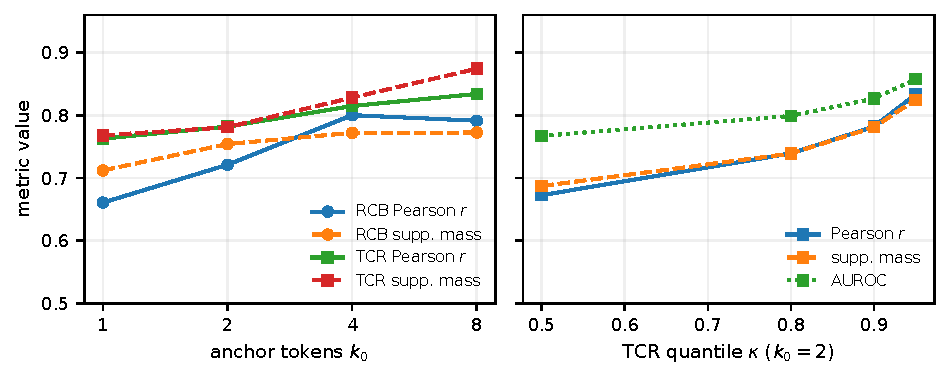
\includegraphics[width=0.85\linewidth]{figures/fig_gatt_sensitivity.pdf}
\caption{Sensitivity of GATT ($v_{\text{logvol}}$, floor-shifted link, $200$ instances). Left: anchor tokens $k_0$ for RCB and TCR ($\kappa = 0.9$). Right: background quantile $\kappa$ for TCR ($k_0 = 2$).}
\label{fig:exp_sensitivity}
\end{figure}

\paragraph{VATT: basis size.}
VATT is insensitive to the number of directions per snippet. With $v_{\text{proj}}$ and $k \in \{1, 2, 4, 8, 16\}$, Pearson $r$ stays at $0.91$, AUROC at $0.92$--$0.93$, MAE at $5.7$--$5.9$\,pp and P@2 at $86.8$--$88.8\%$ (best at $k = 2$). The reason is that the read-outs concentrate on the dominant value directions of the few attended anchor tokens: bases that retain $40\%$, $65\%$, $77\%$ and $87\%$ of the attention-weighted value energy ($k = 1, 4, 8, 16$) already explain $80\%$, $97\%$, $99\%$ and $99.9\%$ of the read-out energy. One pooled read-out vector per snippet (VATT-pool, Section~\ref{subsec:vatt}) is slightly worse with $v_{\text{logvol}}$ ($r = 0.89$, AUROC $0.90$ vs.\ $0.90$ and $0.92$), consistent with Proposition~\ref{prop:set_values}(v).

\begin{table}[t]
\centering
\small
\setlength{\tabcolsep}{3.5pt}
\begin{tabular}{llcccccccccc}
\toprule
 & & \multicolumn{10}{c}{Global layers $g$ ($\ell = 6g - 1$)} \\
\cmidrule(lr){3-12}
$v$ & Layers & 1 & 2 & 3 & 4 & 5 & 6 & 7 & 8 & 9 & 10 \\
\midrule
$v_{\mathrm{proj}}$ & first $g$ & 0.76 & 0.81 & 0.84 & 0.88 & 0.91 & 0.92 & 0.92 & 0.92 & 0.92 & \textbf{0.93} \\
$v_{\mathrm{proj}}$ & only $g$ & 0.76 & 0.84 & 0.87 & 0.91 & \textbf{0.93} & 0.92 & 0.92 & 0.90 & \textbf{0.93} & \textbf{0.93} \\
$v_{\mathrm{logvol}}$ & first $g$ & 0.59 & 0.64 & 0.71 & 0.80 & 0.85 & 0.89 & 0.91 & 0.91 & \textbf{0.92} & 0.91 \\
$v_{\mathrm{logvol}}$ & only $g$ & 0.59 & 0.68 & 0.80 & 0.90 & \textbf{0.95} & 0.93 & 0.94 & 0.89 & 0.93 & 0.90 \\
\bottomrule
\end{tabular}
\caption{Supporting-fact AUROC of VATT ($k = k_r = 8$, floor-shifted link, $200$ instances) when restricting the heads to the first $g$ global layers or to the $g$-th global layer only.}
\label{tab:vatt_layers}
\end{table}

\paragraph{VATT: how many global layers are needed?}
Table~\ref{tab:vatt_layers} restricts VATT to the first $g$ global layers or to a single one. With $v_{\text{proj}}$, the first five global layers ($\ell \le 29$) reach AUROC $0.91$ and P@2 $85.5\%$, the first seven reach AUROC $0.92$ and P@2 $88.0\%$, and the remaining layers add at most $0.01$ AUROC, so extracting values from half of the global layers suffices. The first global layer alone is weak (AUROC $0.76$), and single-layer accuracy peaks in the middle of the network: the fifth global layer ($\ell = 29$) reaches AUROC $0.93$ with $v_{\text{proj}}$ and $0.95$ with $v_{\text{logvol}}$ (P@2 $90.5\%$). Because $v_{\text{logvol}}$ sums per-head mutual informations, it is more sensitive than the energy-weighted $v_{\text{proj}}$ to uninformative early heads (AUROC $0.59$ with the first global layer). The same depth profile appears for the direct attention heuristics (Section~\ref{subsec:exp_citation_easton}).

\subsection{Monte Carlo Error and Cost}
\label{subsec:exp_cost}

\paragraph{Permutation sampling.}
Enumerating all $2^n$ coalitions of the Gram matrix gives the exact Monte Carlo error of the $K$-permutation estimator (Figure~\ref{fig:exp_mc}). The median relative error $\|\bar{\mathbf{m}}_K - \boldsymbol{\Phi}\|_\infty / \|\boldsymbol{\Phi}\|_1$ decays as $K^{-1/2}$, as predicted by Theorem~\ref{thm:bernstein_shapley}. At $K = 100$, it is $1.1\%$ (RCB), $1.4\%$ (EATT) and $2.4\%$ (TCR) for $v_{\text{logvol}}$ (below $0.8\%$ for all three at $K = 1000$), compared with $4.1$--$8.9\%$ for $v_{\text{ent}}$ and up to $30.5\%$ for $v_{\text{vol}}$ on TCR, reflecting the non-negative bounded marginal gains in~\eqref{eq:marginal_logvol}.

\begin{figure}[t]
\centering
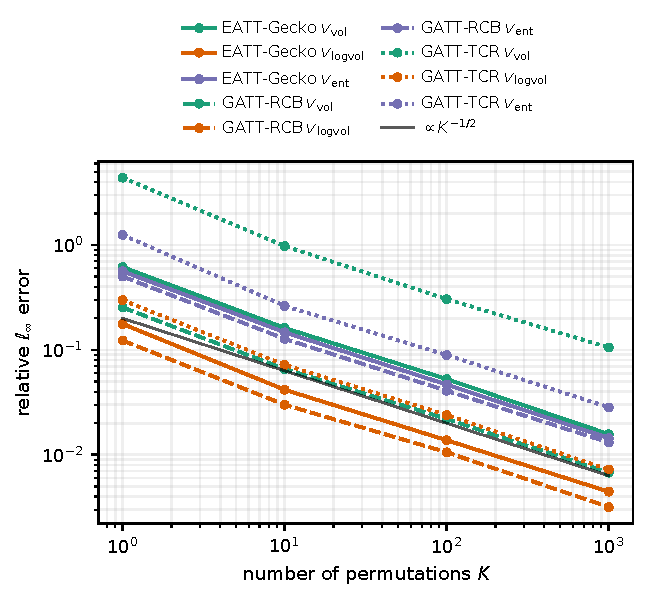
\includegraphics[width=0.58\linewidth]{figures/fig_mc_convergence.pdf}
\caption{Median relative $\ell_\infty$ error of the $K$-permutation Shapley estimator with respect to exact $2^n$ enumeration on the Gram matrix ($n = 6$, $200$ instances). Line style: Gram matrix; color: value function.}
\label{fig:exp_mc}
\end{figure}

\paragraph{Wall-clock cost.}
On $8$ TPU v6e chips, exact $2^n$ likelihood Shapley takes $8.3$\,s per instance ($63.7$ forward passes), $10$-permutation LLH-Shapley $5.7$\,s ($34.9$ distinct passes), and $16$-step Integrated Gradients $8.0$\,s. GATT needs one forward pass on $(p, S, r)$ to extract the global-layer queries, keys and logits ($1.0$\,s), $1.1$\,s to assemble both Gram matrices, and $15$\,ms of CPU time for $K = 100$ permutations across all three value functions. VATT needs one forward pass to extract attention rows and value vectors ($0.94$\,s), $0.48$\,s on the accelerator for the per-head bases and Gram blocks, and about $0.24$\,s of CPU time to tabulate all $64$ coalitions for one configuration; exact Shapley values then take less than $1$\,ms. Including the empty-context pass for $w$, both use two LLM forward passes, independently of $n$ and $K$. EATT needs $n + 1$ encoder calls and $30$\,ms of CPU time and touches the LLM only for $w$.

\paragraph{Answer-correct instances.}
Restricting the evaluation to the $160$ instances with a correct answer leaves every conclusion unchanged within confidence intervals (Appendix~\ref{app:exp_correct}). For example, VATT with $v_{\text{proj}}$ reaches $r = 0.91$, $\rho = 0.79$, MAE $5.8$\,pp, AUROC $0.93$ and P@2 $88.4\%$, and with $v_{\text{vol}}$ (rectified) $\rho = 0.86$, $\tau = 0.81$.


\subsection{Discussion and Limitations}
\label{subsec:exp_discussion}

Even exact likelihood Shapley values inherit the positional sensitivity of causal LLM prompting~\cite{liu2024lost}, so agreement with $v_{\text{LL}}$ complements rather than replaces the supporting-fact evaluation; conversely, supporting-fact labels strictly apply only when the model answers correctly, which is why we repeat all results on the answer-correct instances. All three geometric families explain the observed computation of a single forward pass rather than the counterfactual effect of removing a snippet, which $v_{\text{LL}}$ measures. For VATT, the value vector of a context token is computed from a residual stream that already mixes information from earlier tokens, including other snippets, and information that reaches the response through local attention layers is ignored (Remark~\ref{rem:vatt_limitations}). For $n = 20$, the reference is a $128$-mask ContextCite surrogate, which favors the ContextCite baseline in the agreement metrics; we therefore rely on the supporting-fact labels for MuSiQue and on the label-free LDS and top-$k$ drops for CNN/DailyMail. Our benchmarks stop at $n = 20$ snippets. With a fixed budget, the ablation surrogates already degrade between $n = 6$ and $n = 20$ (KernelSHAP from $r = 0.91$ to $0.61$), while the geometric methods need two passes for any $n$; long-context RAG with hundreds of retrieved chunks, where even a high-budget reference is unavailable, is the natural next test, as are the error-weighted GATT variants of Remark~\ref{rem:error_weighted}.

%%%%%%%%%%%%%%%%%%%%%%%%%%%%%%%%%%%%%%%%%%%%%%%%%%%%%%%%%%%%%%%%%%%%%%%%%%%%%%%%%%%%%%%%%%%%%%%%%%%%%%%%%%%%
\section{Conclusions}
\label{sec:conclusions}

We formulated context attribution for LLMs as a cooperative game whose value functions are defined by the geometry of the snippets and the response rather than by the likelihood of the response under ablated contexts. The three value functions---volume difference, log-volume and spectral entropy---depend only on a Gram matrix, so the same Shapley machinery, link functions and Monte Carlo guarantees apply whatever produces the Gram matrix. The log-volume is the mutual information of a Gaussian channel and coincides with the likelihood game under a power-law likelihood condition, which connects the geometric games to the likelihood-based attribution of~\cite{nematov2025source}. We instantiated the framework with three sources of geometry: an external text encoder (EATT), the query--key routing of the LLM (GATT), and the value subspaces from which the response reads (VATT), for which we extended the value functions from single vectors to sets of vectors via principal angles.

On $200$ HotpotQA instances with Gemma~4 31B and exact $2^n$ likelihood Shapley values as reference, all three families attribute with two LLM passes, independently of the number of snippets. The source of the geometry matters most. EATT and GATT agree with the reference at Pearson $r = 0.72$--$0.78$; VATT, which uses the representations through which the snippets actually influence the response, reaches $r = 0.91$, halves the error to $5.8$ percentage points, matches KernelSHAP with $23$ LLM passes, and exceeds every ablation baseline and the exact reference itself in supporting-fact AUROC ($0.93$). The same conclusions hold on 2WikiMultihopQA ($n = 10$, exact reference), MuSiQue ($n = 20$) and CNN/DailyMail summarization: VATT reaches $r = 0.88$--$0.94$ with two passes, recovers the supporting facts as well as or better than every ablation baseline (AUROC $0.99$ on 2WikiMultihopQA and $0.93$ on MuSiQue), and overtakes fixed-budget KernelSHAP as $n$ grows. With duplicated or paraphrased evidence, the Shapley-based attributions split the credit between the copies, whereas leave-one-out assigns them almost nothing in $35$--$51\%$ of the instances. The log-volume is the robust default across geometries, the volume difference gives the best rankings when every player has an orthonormal basis (Spearman $0.84$ for VATT), and, because components shared by all snippets produce a common offset, the floor-shifted link is needed by every geometric game except the volume difference on VATT, whose redundancy penalty already assigns non-positive credit to the overlapping distractors. Gradient-based attribution of the same likelihood fails because of saturation and off-manifold interpolation, and the first half to two-thirds of the global layers suffice for the attention-based methods.

In practice, we recommend VATT with a few directions per snippet, the mid-network global layers and the floor-shifted link when the generation pass of the model is available---with the projected read-out energy for a handful of snippets and the log-volume when many snippets contribute ($n \ge 20$ or summarization)--- and EATT with the log-volume when only black-box access to the model is possible. Subset-ablation methods remain more accurate when $25$ or more LLM passes per instance are affordable ($r \ge 0.97$). The main open directions are long-context retrieval with hundreds of chunks, where linear-cost ablation becomes prohibitive and even high-budget references are unavailable, and combining the routing (QK) and content (OV) views of attention in a single game.
